%----------------------------------------------------------------------------------------
%	SLIDE 6.
%----------------------------------------------------------------------------------------
\begin{frame}
\frametitle{Hogyan tudjuk megközelíteni az adatokat?}

\pause

\begin{columns}
\begin{column}{0.45\textwidth}
	\begin{block}{Módszerek}
		\begin{itemize}
			\item Machine learning
			\item Machine learning
			\item Machine learning
			\item Machine learning
			\item Machine learning
			\item Machine learning
			\item Machine learning
			\item Machine learning
			\item Machine learning
			\item Machine learning
			\item Machine learning
			\item Machine learning
			\item Machine learning
			\item Machine learning
		\end{itemize}
	\end{block}
\end{column}
\begin{column}{0.45\textwidth}

\pause

\begin{figure}
	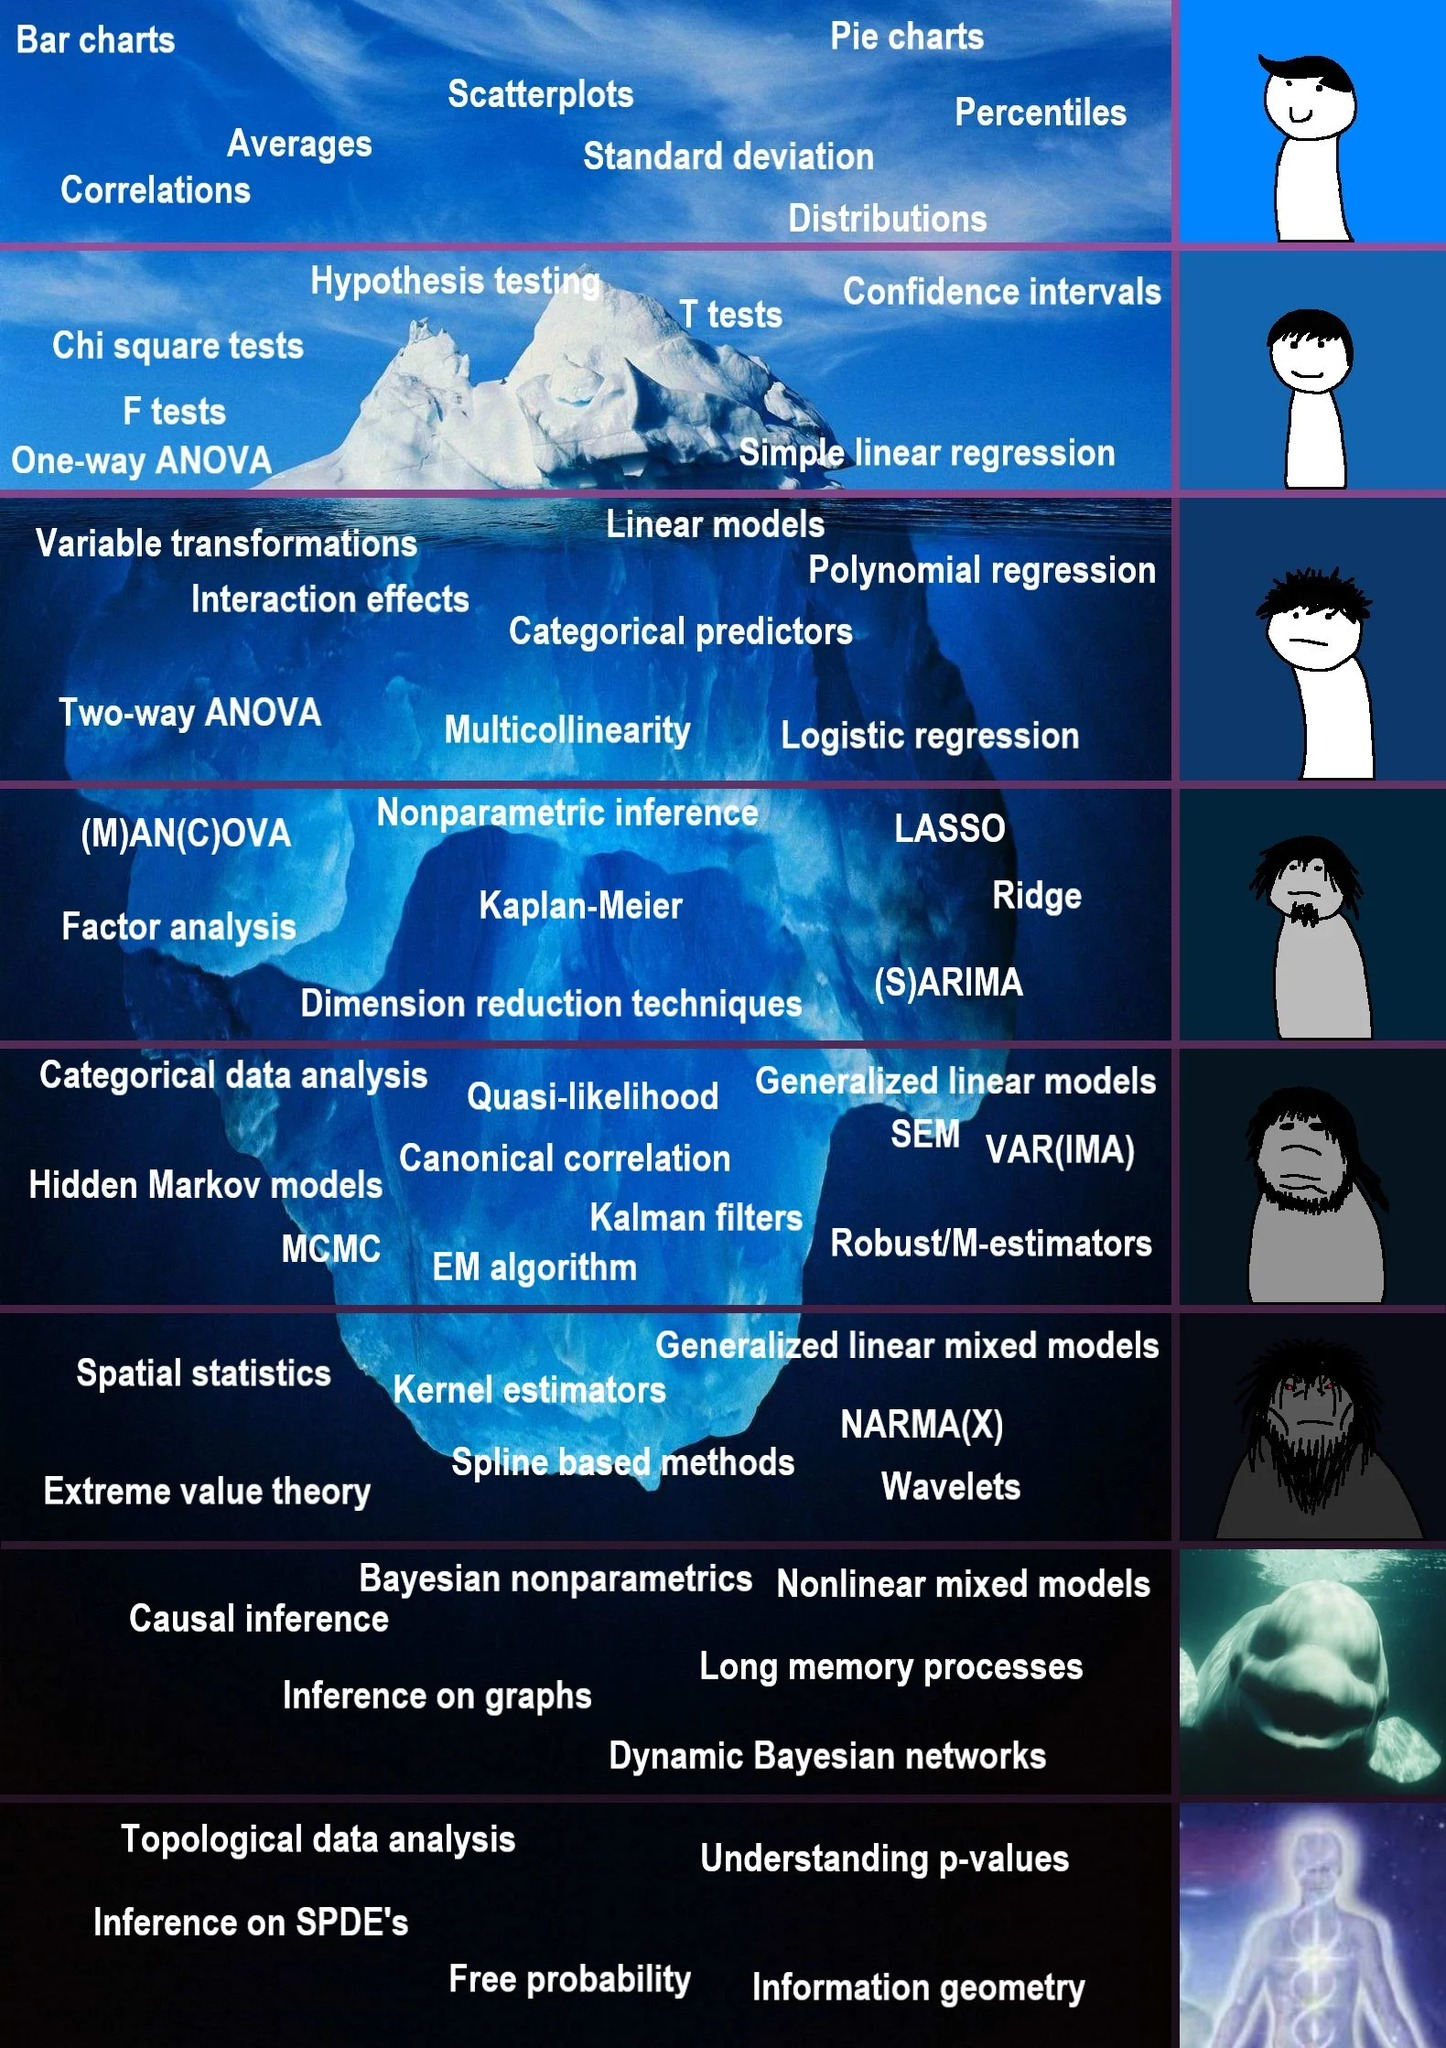
\includegraphics[width=1.0\textwidth]{img/ml.jpg}
\end{figure}
\end{column}
\end{columns}

\end{frame}